\documentclass{article}
\usepackage[utf8]{inputenc}
\usepackage{graphicx}
\usepackage{fancyhdr}
\usepackage{geometry}
\usepackage{amsmath}
\usepackage{amssymb}
\usepackage{url}
\usepackage{hyperref}

\geometry{left = 2.5cm, right=2.5cm, bottom=2.5cm, top=2.5cm}

\title{3806ICT - Week 7 Lab}
\author{Nick van der Merwe - s5151332 - nick.vandermerwe@griffithuni.edu.au}

\pagestyle{fancy}
\renewcommand{\headrulewidth}{1pt}
\fancyhf{}
\rhead{3806ICT - Week 7 Lab}
\chead{Griffith University}
\lhead{Nick van der Merwe - s5151332}
\rfoot{Page \thepage}
\newcommand\tab[1][1cm]{\hspace*{#1}}

\begin{document}
\maketitle

%==============================================================================
\section*{Task 2 - The Bridge Problem}
The fastest way to solve the bridge problem is by 
having the knight and lady go (2 minutes) then the knight back
(2+1=3 minutes) followed by the king and queen (3+10=13mins). 
After this the lady goes back (13+2=15mins) and the knight
and lady cross over to finish (15+2=17mins).
\\
\tab To prove that this is true, we must begin with defining the fields that are
being optimised, primarily the number of crosses - if this is more than the minimum, an
excessive number of crosses were done. Another rule is that the cross back
should always be the fastest person on that side. Firstly, it would be a waste
of time if the king and queen cross separately (i.e. king and knight, knight
back, knight and queen $=> 10+1+5=16$) and that is already next to the maximum.
Furthermore, they are not allowed to cross together at the start as it means
that one of them must come back (king and queen, queen back $=>10+5=15$).
Furthermore, for them to be the only two on the other side at the end it must
mean that one of them crossed back with the torch, or that the torch is still on
the other side. As such, the queen and queen must be the middle pair. As for the
other two pairs, the only option is taking the knight and lady. As such the
first trip are those two, one comes back (can be either, its equal), queen and
king go over as required, and the other first pair crosses back with the torch.
Finally the two fast pairs come back over.
\section*{Task 3 - Explaining PAT}
The first section (lines 4-9) defines the constants using 
$\#define var \leq value \geq$. Max is the most amount of time allowed
KNIGHT is the amount of time it takes for the knight to cross, and so on for
the people. Following this we define vars (lines 11-15) with 
$var varName = \leq value \geq$. These are variables
that can be changed, and these symbolise the side that the
people are on for each person. \\
\tab Next we need to define the processes in lines 17-37 
(usually called models) which has the syntax of 
$processName() = [condition]actionName{action} -> nextProcess [] ...$
. To explain, processName is the name of the process (in our case
South()), and condition is a conditional statement to be allowed
to do the action. Next the actionName is what it prints as 
the action for record and action is what it actually does. Next
we define which process to go to after doing this in nextProcess
and the square brackets essentially functions as a comma between
actions. \\
\tab In line 41 we do $\#define goal(conditional);$ which 
defines the conditional
for when a node is considered succesful which we use in 
$\#assert processName() reaches goal$ on lines 44-46. Essentially, 
this means that the model has a state where a node in the 
search has a state that satisfies the goal. To expand
on this we can pick which node to print using 
$with selection(var)$ in line 46 which picks which node to 
print - in our case we want the minimum.\\
For our output with the minimum time, it looks like this:
\begin{figure}[ht]
    \centering
    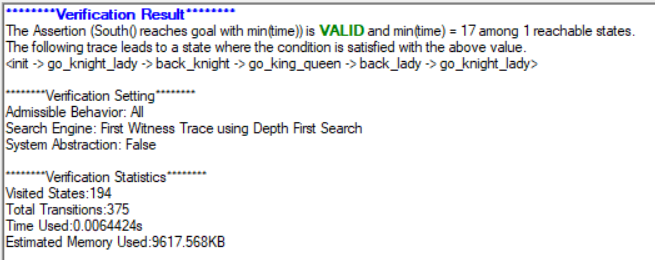
\includegraphics{imgs/verification.png}
\end{figure}

\end{document}
